%-------------------------------------------------------------------------------
% Autores: I. R. Pagnossin e Centro de Ensino e Pesquisa Aplicada.
%
% Este material é parte integrante do curso "Usando LaTeX; pensando em TeX" e é
% distribuido pelos autores segundo a licença Creative Commons 2.5 Brasil
% (atribuição/não-comercial/redistribuição segundo a mesma licença).
%
% This material is part of the course "Usando LaTeX; pensando em TeX".
% It is distributed according to the license Creative Commons 2.5 Brazil
% (attribution/non-comercial use/share alike the same license).
%-------------------------------------------------------------------------------
\newif\ifhandout
%\handouttrue  % Descomente se for para gerar a versão para IMPRESSÃO.
\handoutfalse % Descomente se for para gerar a versão para APRESENTAÇÃO

%-------------------------------------------------------------------------------
\ifhandout
  \documentclass[handout,10pt]{beamer}
  \mode<handout>
\else
	\documentclass[10pt,hyperref={pdfpagelabels=false}]{beamer}
	\mode<presentation>
\fi

	\usepackage[utf8]{inputenc}
	\usepackage{ae}	
	\usepackage[brazil]{babel}	
	\usepackage{graphicx}
	\usepackage{listings}
	\usepackage{tikz}
	\usepackage{amsmath}
	\usepackage[squaren]{SIunits}
	\usepackage{booktabs}
	\usepackage{fancybox}
	\usepackage{array}
	
	\newsavebox{\mybox}
	\savebox{\mybox}{\LARGE$italico$}
	
	\usepackage{bookman}
	%\usepackage{fourier}
	
	\ifhandout
		\usepackage{pgfpages}
		\pgfpagesuselayout{2 on 1}[a4paper,border shrink=5mm]
	\fi

	% Bibliotecas TikZ e PGF necessárias
	\usetikzlibrary{shapes.symbols}
	\usetikzlibrary{calc}
	\usepgflibrary{shapes.misc}
	
	% Configurações pessoais
	% Configurações personalizadas do código LaTeX.	
\lstnewenvironment{LaTeXcode}{
	\setlength{\abovecaptionskip}{0pt}	
	\lstset{language=[LaTeX]TeX}
	\lstset{%
		basicstyle=\footnotesize\ttfamily,  % Global
		keywordstyle=\color{blue}\bfseries, % Comandos
		identifierstyle=,                   % Texto
		stringstyle=,                       % Strings 
		commentstyle=\color{gray},          % Comentários
		showstringspaces=false,             % Espaços
		rulecolor=\color{gray},             % Linha da caixa
	}
	\lstset{emph={setlength,includegraphics,psfrag,subfigure},emphstyle={\color{blue}\bfseries}}
}% Abrindo o ambiente.
{}% Fechando o ambiente.
	
\newcommand{\digite}[1]{{\fontfamily{cmss}\fontseries{bx}\selectfont#1}}	
\newcommand{\cs}[1]{{\normalfont\textbackslash\color{blue!50!black}#1}}
\newcommand{\pkg}[1]{{\normalfont\sffamily\color{orange}#1}}
\newcommand{\env}[1]{{\normalfont\sffamily\color{green!50!black}#1}}
\let\comando=\cs
\let\package=\pkg
\let\ambiente=\env
\newcommand{\foreign}[1]{{\textsl{#1}}}


	\newcounter{exercicio}	
	\newenvironment{exercicio}{%
		\refstepcounter{exercicio}%
		\penalty-200
		\noindent\colorbox{blue!60!black}{\makebox[\columnwidth-\fboxsep*2][c]{\textbf{\color{white}Exercício~\theexercicio}}}\smallskip
	}{\par\medskip}
		

\newcommand{\bibtex}{\textsc{Bib}\TeX}

\newenvironment<>{atividade}[1]{%
\begin{actionenv}#2%
\begin{exampleblock}{{Atividade #1}}%
}
{%
\end{exampleblock}%
\end{actionenv}%
}


	% Path das figuras, relativo a esta pasta.
	\graphicspath{{../arquivos_comuns/figuras/}{./figuras/}}

	% Modelo da apresentação	
	\usetheme{Frankfurt}
	\usefonttheme{serif,structurebold}
	\setbeamercovered{transparent}
		
	\DeclareMathOperator{\sen}{sen}
		
	% Metadados do arquivo PDF.
	\hypersetup{
		pdftitle={Expressões matemáticas I},
		pdfauthor={Dr. Ivan R. Pagnossin},
		pdfsubject={LaTeX},
		pdfkeywords={TeX,LaTeX}
	}

	% Título, autores e instituição.
	\title{Expressões matemáticas I}
	\subtitle{Introdução ao modo matemático}
	\author{\textbf{Prof.:} Ivan R. Pagnossin \and \textbf{Tutora:} Juliana Giordano}
	\institute{%
		Coordenadoria de Tecnologia da Informação\\
		Centro de Ensino e Pesquisa Aplicada}
	\logo{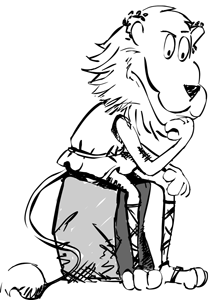
\includegraphics[width=0.25\textwidth]{LogotipoCursoLaTeX_v3_pequeno}}
	\date{}
	
	
	
\begin{document}


%-------------------------------------------------------------------
\begin{frame}[c,label=titulo]
	\centering	
	
	
\includegraphics[width=0.8\textwidth]{LogotipoCursoLaTeX_v2}

	\titlepage
\end{frame}
%-------------------------------------------------------------------
\logo{} % <-- O logotipo não aparecerá mais a partir daqui.
\setbeamertemplate{background canvas}{%
		
\includegraphics[width=\paperwidth,height=\paperheight,keepaspectratio=false]{leao-pensador-wattermark.png}
}

\section{Expressões matemáticas}
\subsection{Estilos de texto e de exibição}
\begin{frame}[fragile]
	\frametitle{O modo matemático}
	\framesubtitle{Estilos de texto e de exibição}

	\begin{block}<1->{Estilo de texto \hfill \foreign{\textbackslash textstyle}}		
		Neste estilo, a expressão matemática aparece no meio do texto, como em \(\boldsymbol{\nabla}\times \boldsymbol{E} =
		- \frac{\partial\boldsymbol{B}}{\partial t}\) (eq.~de Maxwell-Faraday).	
	\end{block}\vfill

	\begin{block}<2->{Estilo de exibição \hfill \foreign{\textbackslash displaystyle}}
	Neste estilo, a expressão matemática tem sua própria linha: \[\oint{\boldsymbol{E}
	\cdot d\boldsymbol{l}} = -\frac{d\Phi}{dt}.\]
	
	\footnotesize\textbf{obs.:} note o ponto-final após a expressão: ela faz parte do texto!
	\end{block}\vfill

	\uncover<3->{%
		\begin{center}
			Observe que a equação no estilo de texto tem extensão vertical menor que aquela no estilo de exibição. \alert<3>{Não lute contra isso!}
		\end{center}}

\end{frame}
%-------------------------------------------------------------------
\subsection{O modo matemático}
\begin{frame}[fragile]
	\frametitle{O modo matemático}
	\framesubtitle{Como começar e terminar}

	\centering

	\begin{columns}
		\column[t]{0.45\textwidth}
		\begin{block}<1->{\centering Estilo de texto}
			\begin{tabular}{rc}
			\LaTeX: & {\color{red}\verb|\(|} \textit{expressão} {\color{red}\verb|\)|} \\
			\TeX:   & {\color{red}\verb|$|}  \textit{expressão} {\color{red}\verb|$|}
			\end{tabular}
		\end{block}
		
		\pause
		\column[t]{0.45\textwidth}
		\begin{block}<2->{\centering Estilo de exibição}
			\begin{tabular}{rc}
			\LaTeX: & {\color{red}\verb|\[|} \textit{expressão} {\color{red}\verb|\]|} \\
			\TeX:   & {\color{red}\verb|$$|} \textit{expressão} {\color{red}\verb|$$|}
			\end{tabular}
		\end{block}
	\end{columns}\vfill
	
	\uncover<3->{\begin{tikzpicture}[node distance=20mm, text height=1.5ex, text depth=0.25ex,
		parmode/.style={rounded rectangle,minimum size=5mm,very thick, draw=green!30, top color=green!20,bottom color=white},
		mathmode/.style={rounded rectangle,minimum size=5mm,very thick, draw=red!30, top color=red!20,bottom color=white},
		tranmode/.style={circle,minimum size=5mm,very thick, draw=black!30, top color=black!20,bottom color=white}]
		\node (text1) [parmode]  {texto};
		\node (tran1) [tranmode,right of=text1] {\textbackslash (};
		\node (expr)  [mathmode,right of=tran1] {\textit{expressão}};
		\node (tran2) [tranmode,right of=expr] {\textbackslash )};
		\node (text2) [parmode,right of=tran2]  {texto};
		
		\draw [->] (text1.east)--(tran1.west);
		\draw [->] (tran1.east)--(expr.west);
		\draw [->] (expr.east)--(tran2.west);
		\draw [->] (tran2.east)--(text2.west);
		
		\node at ($(text1.south) - (0,6mm)$) {\shortstack{modo\\parágrafo}};
		\node at ($(text2.south) - (0,6mm)$) {\shortstack{modo\\parágrafo}};
		\node at ($(expr.south) - (0,6mm)$) {\shortstack{modo\\matemático}};
		\node at ($(tran1.north) + (0,3mm)$) {Transição};
		\node at ($(tran2.north) + (0,3mm)$) {Transição};
	\end{tikzpicture}}\vfill
	
	\begin{enumerate}
	\item<4-> As regras do modo matemáticos são diferentes
	\item<5-> Instruções de um modo não necessariamente funcionam no outro
	\footnotesize(eg, \verb|_| e \verb|^| só funcionam no modo matemático)
	\end{enumerate}
		
\end{frame}
%-------------------------------------------------------------------
\begin{frame}
	\frametitle{O modo matemático}
	\framesubtitle{Convenção de forma das fontes}

	\begin{itemize}
	\item<1-> Números e símbolos têm \emph{forma} (NFSS) ``\textrm{normal}''
	\item<2-> Variáveis têm \emph{forma} (NFSS) ``\textit{itálico}''
	\end{itemize}\vfill
	
	\[
		\alert<1>{\int}_{\alert<2>{\phi} \alert<1>{= 0}}^{\alert<1>{2}\alert<2>{\pi}} \alert<1>{\int}_{\alert<2>{\theta} \alert<1>{= 0}}^{\alert<2>{\pi}} \alert<2>{Y}_{\alert<2>{n}_{\alert<1>{1}}}^{\alert<2>{m}_{\alert<1>{1*}}} \alert<1>{(}\alert<2>{\theta}\alert<1>{,}\alert<2>{\phi}\alert<1>{)} \alert<2>{Y}_{\alert<2>{n}_{\alert<1>{2}}}^{\alert<2>{m}_{\alert<1>{2}}} \alert<1>{(}\alert<2>{\theta}\alert<1>{,}\alert<2>{\phi}\alert<1>{)}
		\alert<1>{\sin}\alert<2>{\theta}\, \alert<2>{d\theta\, d\phi} \alert<1>{=} \alert<2>{\delta}_{\alert<2>{n}_{\alert<1>{1}} \alert<2>{n}_{\alert<1>{2}}} \alert<2>{\delta}_{\alert<2>{m}_{\alert<1>{1}} \alert<2>{m}_{\alert<1>{2}}}
	\]\vfill
	
	\begin{description}
		\item<3->[\textbf{Atenção:}] as fontes dos modos matemático e parágrafo não são necessariamente as mesmas
		\item<4->[\textbf{Cuidado:}] jamais use o modo matemático para escrever em itálico! Veja:
		
		\bigskip
		
		$\underset{\text{\footnotesize correto}}{\text{\fontfamily{cmr}\selectfont\LARGE\textit{itálico}}}$
		\quad vs.\quad 
		\visible<4->{$\underset{\text{\footnotesize incorreto}}{\usebox{\mybox}}$}.
	\end{description}
	
\end{frame}
%-------------------------------------------------------------------
\subsection{Regras do modo matemático}
\begin{frame}[fragile]
	\frametitle{O modo matemático}
	\framesubtitle{As 3 regras básicas}
			
	\begin{enumerate}
	\item<2-> Espaços (e quebras de linha) são ignorados\\
	          \uncover<3->{\footnotesize\textbf{dica:} organize a expressão de modo a facilitar a visualização.}
	\item<4-> Linhas em branco (mudança de parágrafo) são proibidas
	\item<5-> Acentos são proibidos
	\end{enumerate}
	
	\vspace*{\stretch{1}}	

	\begin{atividade}<6->{1}
		\begin{LaTeXcode}
			\(a  +  b  =  c\) e \(a+b=c\) são equivalentes.
		\end{LaTeXcode}
	\end{atividade}

	\vspace*{\stretch{1}}

	\begin{uncoverenv}<7->
		\begin{center}	
			\footnotesize
			\begin{tikzpicture}[text height=1.5ex, text depth=0.25ex,
				parmode/.style={rounded rectangle,minimum size=5mm,very thick, draw=green!30, top color=green!20,bottom color=white},
				mathmode/.style={rounded rectangle,minimum size=5mm,very thick, draw=red!30, top color=red!20,bottom color=white},
				tranmode/.style={circle,minimum size=5mm,very thick, draw=black!30, top color=black!20,bottom color=white}]
				
				\node (text1) [node distance=15mm]{};
				\node (expr1) [mathmode,right of=text1,node distance=10mm] {a + b = c};
				\node (text2) [parmode,right of=expr1,node distance=15mm]  {\textvisiblespace e\textvisiblespace};
				\node (expr2) [mathmode,right of=text2,node distance=15mm] {a+b=c};
				\node (text3) [parmode,right of=expr2,node distance=25mm]  {\textvisiblespace são\textvisiblespace equivalentes.};
				\node (text4) [right of=text3,node distance=20mm] {};
						
				\draw [->] (text1.east)--(expr1.west);
				\draw [->] (expr1.east)--(text2.west);
				\draw [->] (text2.east)--(expr2.west);
				\draw [->] (expr2.east)--(text3.west);
				\draw [->] (text3.east)--(text4.west);
			\end{tikzpicture}
		\end{center}
	\end{uncoverenv}
	
	\vspace*{\stretch{1}}
	
	\begin{block}<8->{Exercício 1\hspace*{\stretch{1}}\hyperlink{respostas1-8}{\footnotesize\textbf{(resposta)}}}
	O que acontece se transferirmos os espaços ao redor da letra ``e'' para os modos matemáticos adjacentes?
	\end{block}
	
\end{frame}
%-------------------------------------------------------------------
\subsection{Operações aritméticas}
\begin{frame}[fragile]
	\frametitle{Operações aritméticas}
	
	\small
	
	\begin{atividade}{2}
		\begin{tabbing}
		\hspace*{0.3\textwidth}: \=\kill
		\onslide<1->{\textcolor{blue!60}{Soma:}}           \> \begin{uncoverenv}<1->\verb|a + b|\end{uncoverenv}
		                                                      \`\onslide<1->{\( a + b \)}                        \\[1ex]
		\onslide<2->{\textcolor{red!60}{Subtração:}}       \> \begin{uncoverenv}<2->\verb|a - b|\end{uncoverenv}
		                                                      \`\onslide<2->{\( a - b \)}                        \\[1ex]
		\onslide<3->{\textcolor{green!60}{Multiplicação:}} \> \begin{uncoverenv}<3->\verb|ab|\end{uncoverenv}
		                                                      \`\onslide<3->{\(a b\)}                            \\
		                                                   \> \begin{uncoverenv}<3->\verb|a\cdot b|\end{uncoverenv}
		                                                      \`\onslide<3->{\( a\cdot b \)}                     \\[1ex]
		\onslide<4->{\textcolor{black!60}{Divisão:}}       \> \begin{uncoverenv}<4->\verb|a/b|\end{uncoverenv}
		                                                      \`\onslide<4->{\( a/b \)}                          \\
		                                                   \> \begin{uncoverenv}<4->\verb|\frac{a}{b}|\end{uncoverenv}
		                                                      \`\onslide<4->{\(\displaystyle\frac{a}{b}\)}
		\end{tabbing}
	\end{atividade}
	
	\vspace*{\stretch{1}}
		
	\begin{block}<5->{Exercício 2\hspace*{\stretch{1}}\hyperlink{respostas1-8}{\footnotesize\textbf{(resposta)}}}
		Reproduza a expressão abaixo no \alert<5>{estilo de exibição}.
		\[\displaystyle \frac{a\cdot b - c}{d + e/f}\]
		
	\footnotesize\textbf{Dica:} monte a expressão em passos pequenos.
	\end{block}
	
	\vspace*{\stretch{1}}
	
	\begin{center}
		\begin{actionenv}<3-|alert@3>
			\textbf{Atenção:} não escreva \verb|a.b|, \verb|a * b| ou \verb|a x b|!
		\end{actionenv}
	\end{center}
	
\end{frame}
%-------------------------------------------------------------------
\subsection{Subscritos e sobrescritos}
\begin{frame}[fragile,c]
	\frametitle{Subscritos e sobrescritos}
			
	\begin{atividade}{2}
		\begin{columns}
			\column[t]<1->{0.45\textwidth}
			\begin{tabular}{l!{\footnotesize produz}>{\(}l<{\)}}
				\verb|a_{b}|     & a_{b}     \\
				\verb|a_{bc}|    & a_{bc}    \\
				\verb|a_{b_{c}}| & a_{b_{c}}
			\end{tabular}

			%-------------------------					
			\column[t]<3->{0.45\textwidth}
			\begin{tabular}{l!{\footnotesize produz}>{\(}l<{\)}}
				\verb|a^{b}|     & a^{b}     \\
				\verb|a^{bc}|    & a^{bc}    \\
				\verb|a^{b^{c}}| & a^{b^{c}}
			\end{tabular}
		\end{columns}
	\end{atividade}
			
	\vspace*{\stretch{1}}
			
	\begin{columns}
		\column[t]{0.45\textwidth}		
			\begin{block}<2->{Exercício 3\hspace*{\stretch{1}}\hyperlink{respostas1-8}{\footnotesize\textbf{(resposta)}}}
				\[A_n + B_{nm} + C_{n_m}\]
			\end{block}
		%-------------------------	
		\column[t]{0.45\textwidth}		
			\begin{block}<4->{Exercício 4\hspace*{\stretch{1}}\hyperlink{respostas1-8}{\footnotesize\textbf{(resposta)}}}
				\[A^n + B^{nm} + C^{n^m}\phantom{C_{n_m}}\]
			\end{block}
	\end{columns}
	
	\vspace*{\stretch{1}}
	
	\begin{block}<5->{Exercício 5\hspace*{\stretch{1}}\hyperlink{respostas1-8}{\footnotesize\textbf{(resposta)}}}
		\[A_n^n + B_{nm}^{nm} + C_{n_m}^{n^m}\]
	\end{block}
	
	\vspace*{\stretch{1}}
	
	\begin{center}
		\begin{actionenv}<1-|alert@1>
			\textbf{Atenção:} cuidado para não escrever \verb|a^b^c| ou \verb|a_b_c|
		\end{actionenv}
	\end{center}
	
\end{frame}
%-------------------------------------------------------------------
\subsection{Integrando texto e expressões}
\begin{frame}[fragile]
	\frametitle{Integrando texto e expressões}
	
	\begin{block}<1->{Exercício 6\hspace*{\stretch{1}}\hyperlink{respostas1-8}{\footnotesize\textbf{(resposta)}}}
		Produza um documento com o seguinte texto:
		
		\medskip
		
		{\small Segundo o teorema de Fermat, a equação \(a^n = b^n + c^n\)
		só tem solução para \(n \le 2\), sendo \(a\), \(b\), \(c\)
		e \(n\) números inteiros não nulos.}
		
		\bigskip
		
		\footnotesize\textbf{obs.:} utilize \verb|\le| para produzir \(\le\).
	\end{block}
	
	\vspace*{\stretch{1}}
	
	\begin{atividade}<2->{3}
		\begin{LaTeXcode}
			texto \(\displaystyle \frac{1}{2}\) texto\par			
			texto \[\textstyle \frac{1}{2}\] texto
		\end{LaTeXcode}
	\end{atividade}
	
	\vspace*{\stretch{1}}
	
	\begin{center}%	
		\begin{actionenv}<2-| alert@2>%			
			\textbf{Atenção:} pense duas vezes antes de usar\\\verb|\textstyle| ou \verb|\displaystyle|			
		\end{actionenv}%
	\end{center}	
	
\end{frame}
%-------------------------------------------------------------------
\subsection{Delimitadores}
\begin{frame}[fragile]
	\frametitle{Controle automático de delimitadores}
		
	\begin{atividade}{4}
		\begin{itemize}
			\item<1-> \verb|(\frac{a}{b})^2| \hfill \(\displaystyle(\frac{a}{b})^2\)
		\end{itemize}
		
		\vspace*{\stretch{1}}
		
		\begin{center}
			{\color{blue}\verb|(|}\textit{expressão}{\color{red}\verb|)|} \pause\quad\(\to\)\quad
			{\color{blue}\verb|\left(|}\textit{expressão}{\color{red}\verb|\right)|}
		\end{center}
		
		\vspace*{\stretch{1}}
			
		\begin{itemize}
			\item<4-> {\color{blue}\verb|\left(|}\verb|  \frac{a}{b} |{\color{red}\verb|\right)|}\verb|^2|%
								\hfill \(\displaystyle\left(\frac{a}{b}\right)^2\)
			\item<5-> {\color{blue}\verb|\left\{|}\verb| \frac{a}{b} |{\color{red}\verb!\right|!}\verb|^2|%
								\hfill \(\displaystyle\left\{\frac{a}{b}\right|^2\)
			\item<6-> {\color{blue}\verb|\left.|}\verb|  \frac{a}{b} |{\color{red}\verb|\right]|}\verb|^2|%
								\hfill \(\displaystyle\left.\frac{a}{b}\right]^2\)
		\end{itemize}
		
	\end{atividade}
	
	\vspace*{\stretch{1}}
	
	\uncover<7->{\begin{center}
		\footnotesize\hyperlink{delimitadores}{Clique aqui para ver a lista completa de delimitadores}
	\end{center}}
\end{frame}
%-------------------------------------------------------------------
\begin{frame}[fragile]
	\frametitle{Exercícios}

	\begin{columns}
		\column[t]{0.45\textwidth}
		\begin{block}{Exercício 7\hspace*{\stretch{1}}\hyperlink{respostas1-8}{\footnotesize\textbf{(resposta)}}}
		\[a^{bc} \ne a^bc\]		
		\footnotesize\textbf{obs.:} use \verb|\ne| para produzir \(\ne\).
		\end{block}
		
		\column[t]{0.45\textwidth}
		\begin{block}{Exercício 8\hspace*{\stretch{1}}\hyperlink{respostas1-8}{\footnotesize\textbf{(resposta)}}}
		\[\frac{a^{2b} + \sqrt[7]{ab}}{a^{2^b}}\]
		\end{block}		
	\end{columns}

	\vspace*{\stretch{1}}

	\begin{block}{Exercício 9\hspace*{\stretch{1}}\hyperlink{respostas9-13}{\footnotesize\textbf{(resposta)}}}
		\[
			dl = \sqrt[2]{1 + \left( \frac{dy}{dx} \right)^2} dx
		\]
	\end{block}
	
	\vspace*{\stretch{1}}
	
	\begin{block}{Exercício 10\hspace*{\stretch{1}}\hyperlink{respostas9-13}{\footnotesize\textbf{(resposta)}}}
		\[
			\left[ \frac{x^2 - y^2}{ \left( x + y \right)^2 } \right]^2 =
		  \left[ \frac{\left(x - y\right)\left(x + y\right)}{ \left( x + y \right)^2 } \right]^2 =
		  \frac{\left(x - y\right)^2}{ \left( x + y \right)^2 }
		\]%
	\end{block}

\end{frame}
%-------------------------------------------------------------------
\subsection{Reticências}
\begin{frame}[fragile]
	\frametitle{Reticências}	
	
	\begin{itemize}
		\item<1-> \verb|\ldots| (\foreign{lower dots})    \hfill {\LARGE\(\ldots\)}
		\item<2-> \verb|\cdots| (\foreign{centered dots}) \hfill {\LARGE\(\cdots\)}
		\item<3-> \verb|\vdots| (\foreign{vertical dots}) \hfill {\LARGE\(\vdots\)}
		\item<4-> \verb|\ddots| (\foreign{diagonal dots}) \hfill {\LARGE\(\ddots\)}
	\end{itemize}
	
	\vspace*{\stretch{1}}
	
	\begin{center}
		\onslide<1->{\alert<6>{\(a_1, a_2, \ldots, a_n\)}}\hfill
		\onslide<2->{\alert<6>{\(a_1 + a_2 + \cdots + a_n\)}}\hfill
		\onslide<3->{\(\begin{matrix}a_1\\ \vdots\\ a_n\end{matrix}\)}\hfill
		\onslide<4->{\(\begin{matrix}a_1 & & \\ &\ddots&\\ & &a_n\end{matrix}\)}
	\end{center}
	
	\vspace*{\stretch{1}}
	
	\begin{block}<5->{Exercício 11\hspace*{\stretch{1}}\hyperlink{respostas9-13}{\footnotesize\textbf{(resposta)}}}
			Produza as duas expressões \alert{destacadas}.
	\end{block}
	
\end{frame}
%-------------------------------------------------------------------
\subsection{Referências cruzadas}
\begin{frame}[fragile]
	\frametitle{Referências cruzadas}
	\framesubtitle{\textcolor{green}{Atividade 5}}
		
	\begin{columns}
		\column[T]{0.35\textwidth}
		\begin{LaTeXcode}
			\begin{equation}
			  a^2 = b^2 + c^2
			\end{equation}		
		\end{LaTeXcode}
		%-------------------------
		\column[T]{0.60\textwidth}
		\small A eq. tem número, mas não tem \textbf{nome}			
		\begin{equation}
		  \label{eq:pitagoras}
		  a^2 = b^2 + c^2
		\end{equation}		
	\end{columns}
	
	\vspace*{\stretch{1}}
	
	\begin{block}<2->{}
		\centering
		\cs{label}\{\alert<2>{\textit{nome}}\}
	\end{block}
	
	\vspace*{\stretch{1}}
	
	\begin{uncoverenv}<3->
		\begin{columns}
			\column[T]{0.35\textwidth}
			\begin{LaTeXcode}
				\begin{equation}
				\label{eq:pitagoras}
				a^2 = b^2 + c^2
				\end{equation}		
			\end{LaTeXcode}
			%-------------------------
			\column[T]{0.60\textwidth}		
			 A eq. agora tem nome: ``\textit{eq:pitagoras}''
			\begin{equation}
			\label{eq:pitagoras}
			a^2 = b^2 + c^2
			\end{equation}		
		\end{columns}
	\end{uncoverenv}
	
	\vspace*{\stretch{1}}
	
	\begin{block}<4->{}
		\centering
		\hfill\cs{ref}\{\alert<4>{\textit{nome}}\}\hfill ou\hfill \cs{eqref}\{\alert<4>{\textit{nome}}\} (\pkg{amsmath})\hfill{}
	\end{block}
	
	\vspace*{\stretch{1}}
	
	\begin{itemize}
		\item<5-> Arquivo auxiliar (\texttt{aux})
		\item<6-> Equações, figuras, seções, capítulos, páginas, \dots
	\end{itemize}
	
\end{frame}
%-------------------------------------------------------------------
\subsection{Derivadas e diferenciais}
\begin{frame}[fragile]
	\frametitle{Derivadas e diferenciais}
		
	\animate<2-9>
	\begin{atividade}{6}
		\begin{itemize}
			\item<2-> \verb|y'|       \hfill \(y'\)
			\item<3-> \verb|y''|      \hfill \(y''\)
			\item<4-> \verb|y'''|     \hfill \(y'''\)
			\item<5-> \verb|\dot y|   \hfill \(\dot y\)
			\item<6-> \verb|\ddot y|  \hfill \(\ddot y\)
			\item<7-> \verb|\dddot y| \hfill \(\dddot y\)
			\item<8-> \verb|y^{(n)}|  \hfill \(y^{(n)}\)
			\item<9-> \verb|\partial| \hfill \(\partial\)
		\end{itemize}
	\end{atividade}
	
	\vspace*{\stretch{1}}
	
	\begin{block}<10->{Exercício 12\hspace*{\stretch{1}}\hyperlink{respostas9-13}{\footnotesize\textbf{(resposta)}}}
		Reproduza a expressão abaixo no estilo de exibição:
	
		\[\frac{dy}{dt} = \dot x \, \frac{\partial y}{\partial x} + \frac{\partial y}{\partial t}\]
	\end{block}
	
\end{frame}
%-------------------------------------------------------------------
\subsection{Integrais e somatórias}
\begin{frame}[fragile]
	\frametitle{Integrais, somatórios e produtórios}
	
	\animate<2-5>
	\begin{atividade}{6}
		\begin{itemize}
			\item<2-> \verb|\int|\quad \verb|\iint|\quad \verb|\oint| \hfill \(\int \quad \iint \quad \oint\)
			\item<3-> \verb|\sum_{i}^{n} x_i| \hfill \(\sum_{i}^{n} x_i\)
			\item<4-> \verb|\prod_{i}^{n} x_i| \hfill \(\prod_{i}^{n} x_i\)
			\item<5-> \verb|\int_{0}^{1} a\, dx| \hfill \(\int_{0}^{1} a\, dx\)
			\item<6-> \verb|\int\limits_{0}^{1} a\, dx| \hfill \(\int\limits_0^1 a\, dx\)
		\end{itemize}
	\end{atividade}
	
	\vspace*{\stretch{1}}
	
	\begin{block}<7->{Exercício 13\hspace*{\stretch{1}}\hyperlink{respostas9-13}{\footnotesize\textbf{(resposta)}}}
		Reproduza a expressão abaixo no estilo de exibição:
		
		\[\int_0^\infty f(x)\, dx \approx \sum_{i = 1}^n w_i e^{x_i} f(x_i)\]
		
		\footnotesize\textbf{obs.:} use \verb|\infty| para \(\infty\) e \verb|\approx| para \(\approx\).
	\end{block}
	
\end{frame}
%-------------------------------------------------------------------
\subsection{Nomes de funções}
\begin{frame}[fragile]
	\frametitle{Nome de funções}
		
	\begin{tabular}{lll}
		\verb|\sin| & \verb|\arcsin| & \verb|\sinh| \\
		\verb|\cos| & \verb|\arccos| & \verb|\cosh| \\
		\verb|\tan| & \verb|\arctan| & \verb|\tanh| \\
		\verb|\log| & \verb|\ln|     & \verb|\exp|
	\end{tabular}\hfill
	\begin{tabular}{lll}
		$\sin$ & $\arcsin$ & $\sinh$ \\
		$\cos$ & $\arccos$ & $\cosh$ \\
		$\tan$ & $\arctan$ & $\tanh$ \\
		$\log$ & $\ln$     & $\exp$
	\end{tabular}
	
	\vspace*{\stretch{1}}
	
	\begin{block}<2->{Como escrever $\sen$ ao invés de $\sin$ (e similares)?\dots}
		\cs{DeclareMathOperator}\{\verb|\comando|\}\{\textit{nome}\}\\[0.5cm]
		
		\footnotesize
		\textbf{obs. 1:} só pode ser utilizado no preâmbulo.\\
		\textbf{obs. 2:} requer o pacote \pkg{amsmath}.
	\end{block}
	
	\vspace*{\stretch{1}}
	
	\begin{atividade}<3->{7}	
		\[\sen^2\phi + \cos^2\phi = 1\]
	\end{atividade}		
\end{frame}
%-------------------------------------------------------------------
\subsection{Texto no modo matemático}
\begin{frame}[fragile]
	\frametitle{Fontes no modo matemático}
	
	\uncover<1->{Para inserir texto \emph{dentro} de uma expressão, use:}
	\begin{columns}
		\column{\textwidth}
		\begin{itemize}
		\item<1-> \verb|\mbox| ou \verb|\text| (\pkg{amsmath}) e
		\item<2-> \verb|\text|\textcolor{red}{\textit{xx}}
		\end{itemize}
	\end{columns}
	
	\bigskip
	
	\animate<3-7>
	\uncover<3->{Para mudar a fonte de um símbolo numa expressão, use:}
	\begin{columns}
		\column{0.45\textwidth}
		\begin{itemize}
		\item<3-> \verb|\mathrm|\hfill \(\mathrm{ABCD}\)
		\item<4-> \verb|\mathsf|\hfill \(\mathsf{ABCD}\)
		\item<5-> \verb|\mathtt|\hfill \(\mathtt{ABCD}\)
		\item<6-> \verb|\mathbf|\hfill \(\mathbf{ABCD}\)
		\item<7-> \verb|\mathit|\hfill \(\mathit{ABCD}\)
		\item<8-> \verb|\mathcal|\hfill \(\mathcal{ABCD}\)	
		\end{itemize}
		
		\column[c]{0.45\textwidth}
		\centering		
		\begin{atividade}<9->{8}\centering	
			texto \( \cos\left(\phi_{\mbox{médio}}\right) \) texto\\
			texto \( \cos\left(\phi_{\textbf{médio}}\right) \) texto\\			
			texto \( \cos\left(\phi_{\text{médio}}\right) \) texto\\	
			texto \( \cos\left(\mathcal{A}\right) \) texto
		\end{atividade}	
	\end{columns}
	
	\bigskip
	
	\begin{uncoverenv}<8->
	\centering
	\textbf{Atenção:} não use \verb|\math|\textcolor{red}{\textit{xx}} para \emph{escrever} no modo matemático
	\end{uncoverenv}
			
\end{frame}
%-------------------------------------------------------------------
{
	\logo{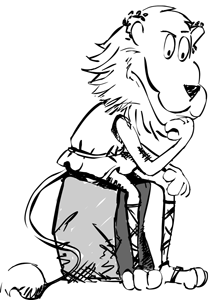
\includegraphics[width=0.25\textwidth]{LogotipoCursoLaTeX_v3_pequeno}}
	\setbeamertemplate{background canvas}{}
	\againframe{titulo} % Reapresenta a página inicial.
}
%-------------------------------------------------------------------
%-------------------------------------------------------------------
%-------------------------------------------------------------------
\section{Apêndice}
\subsection{Delimitadores}
\begin{frame}[fragile,label=delimitadores]
	\frametitle{Delimitadores aceitos por {\ttfamily \textbackslash left} e {\ttfamily \textbackslash right}}

	\centering
	
	\begin{tabular}{l>{\(}l<{\)}|l>{\(}l<{\)}}
		\verb|(|                          & (            & \verb|)|                         & ) \\
		\verb|[|                          & [            & \verb|]|                         & ] \\
		\verb|\{|                         & \{           & \verb|\}|                        & \} \\
		\verb!|! ou \verb|\vert|          & |            & \verb!\|! ou \verb|\Vert|        & \| \\
		\verb|/|                          & /            & \verb|\backslash|                & \backslash \\		
		\verb|\lfloor|                    & \lfloor      & \verb|\rfloor|                   & \rfloor \\
		\verb|\lceil|                     & \lceil       & \verb|\rceil|                    & \rceil \\
		\verb|\langle|                    & \langle      & \verb|\rangle|                   & \rangle \\
		\verb|\uparrow|                   & \uparrow     & \verb|\downarrow|                & \downarrow \\
		\verb|\Uparrow|                   & \Uparrow     & \verb|\Downarrow|                & \Downarrow \\
		\verb|\updownarrow|               & \updownarrow & \verb|\Updownarrow|              & \Updownarrow \\
		\verb|\ulcorner| (\pkg{amsmath})  & \ulcorner    & \verb|\urcorner| (\pkg{amsmath}) & \urcorner \\
		\verb|\llcornder| (\pkg{amsmath}) & \llcorner    & \verb|\lrcorner| (\pkg{amsmath}) & \lrcorner \\
		\verb|.|                          & \textit{vazio}
 	\end{tabular}\vfill

	\footnotesize
	\textbf{obs.:} os comandos marcados com \pkg{amsmath} requerem o pacote \emph{amsmath}.

\end{frame}
%-------------------------------------------------------------------
\subsection{Respostas}
\begin{frame}[fragile,label=respostas1-8]
	\frametitle{Respostas}
	\scriptsize
	
	\begin{enumerate}
	\item Somem os espaços entre ``e'' e as expressões porque os espaços, no modo matemático, são ignorados.
	
	\item%
		\begin{LaTeXcode}
		\[\frac{a\cdot b - c}{d + e/f}\]
		\end{LaTeXcode}
		
	\item%
		\begin{LaTeXcode}
		\[A_n + B_{nm} + C_{n_m}\]
		\end{LaTeXcode}
		
	\item%
		\begin{LaTeXcode}
		\[A^n + B^{nm} + C^{n^m}
		\end{LaTeXcode}
		
	\item%
		\begin{LaTeXcode}
		\[A_n^n + B_{nm}^{nm} + C_{n_m}^{n^m}\]
		\end{LaTeXcode}
		
	\item%
		\begin{LaTeXcode}
		Segundo o teorema de Fermat, a equação \(a^n = b^n + c^n\)
		só tem solução para \(n \le 2\), sendo \(a\), \(b\), \(c\)
		e \(n\) números inteiros não nulos.
		\end{LaTeXcode}
		
	\item%
		\begin{LaTeXcode}
		\[a^{bc} \ne a^bc\]
		\end{LaTeXcode}
		
	\item%
		\begin{LaTeXcode}
		\[\frac{a^{2b} + \sqrt[7]{ab}}{a^{2^b}}\]
		\end{LaTeXcode}
		
	\end{enumerate}

\end{frame}
%-------------------------------------------------------------------
\begin{frame}[fragile,label=respostas9-13]
	\frametitle{Respostas}
	\scriptsize
	
	\begin{enumerate}\setcounter{enumi}{8}
	\item%
		\begin{LaTeXcode}
		\[dl = \sqrt[2]{1 + \left( \frac{dy}{dx} \right)^2} dx\]
		\end{LaTeXcode}	
	
	\item%
		\begin{LaTeXcode}
		\[\left[ \frac{x^2 - y^2}{ \left( x + y \right)^2 } \right]^2
		=	\left[ \frac{\left(x - y\right)\left(x + y\right)}{ \left(
		x +	y \right)^2 } \right]^2 =	\frac{\left(x - y\right)^2}{
		\left( x + y \right)^2 }\]
		\end{LaTeXcode}
		
	\item%
		\begin{LaTeXcode}
		\(a_1, a_2, \ldots, a_n\)
		\end{LaTeXcode} e
		\begin{LaTeXcode}
		\(a_1 + a_2 + \cdots + a_n\)
		\end{LaTeXcode}
		
	\item%
		\begin{LaTeXcode}
		\[\frac{dy}{dt} = \dot x \, \frac{\partial y}{\partial x} 
		+ \frac{\partial y}{\partial t}\]
		\end{LaTeXcode}
		
	\item%
		\begin{LaTeXcode}
		\[\int_0^\infty f(x)\, dx \approx \sum_{i = 1}^n w_i
		e^{x_i} f(x_i)\]
		\end{LaTeXcode}
	\end{enumerate}
	
\end{frame}
\end{document}